%% 附录第一章--app1.tex
\chapter{这里是附录}\label{app:1}
未尽事宜可将其列在附录中加以说明。论文有关的数据表、符号说明、计算程序、运行结果、
主要设备、仪器仪表的性能指标和测试分析结果、精度等均可列在附录中。
\section{附录的节}
与正文类似。
\begin{table}[ht]
	\centering
	\caption{测试表格}\label{tab:mytable}
	\begin{tabular}{cc}
		\toprule
		a & B   \\
		\midrule
		甲   & 乙丙丁 \\
		\bottomrule
	\end{tabular}
\end{table}

\subsection{附录的小节}
\zhlipsum[1][name = zhufu]

\begin{figure}[ht]
	\centering
	\begin{minipage}{0.4\textwidth}
		\centering
		
\includegraphics[height=4cm]{image-a.pdf}
		\caption{第一张图}\label{fig:test1}
	\end{minipage}
	\hspace{1cm}
	\begin{minipage}{0.4\textwidth}
		\centering
		
\includegraphics[height=4cm]{image-c.pdf}
		\caption{第二张图}\label{fig:test2}
	\end{minipage}
\end{figure}

\zhlipsum[name = xiangyu]

\begin{dfigure}[tbp]
	\centering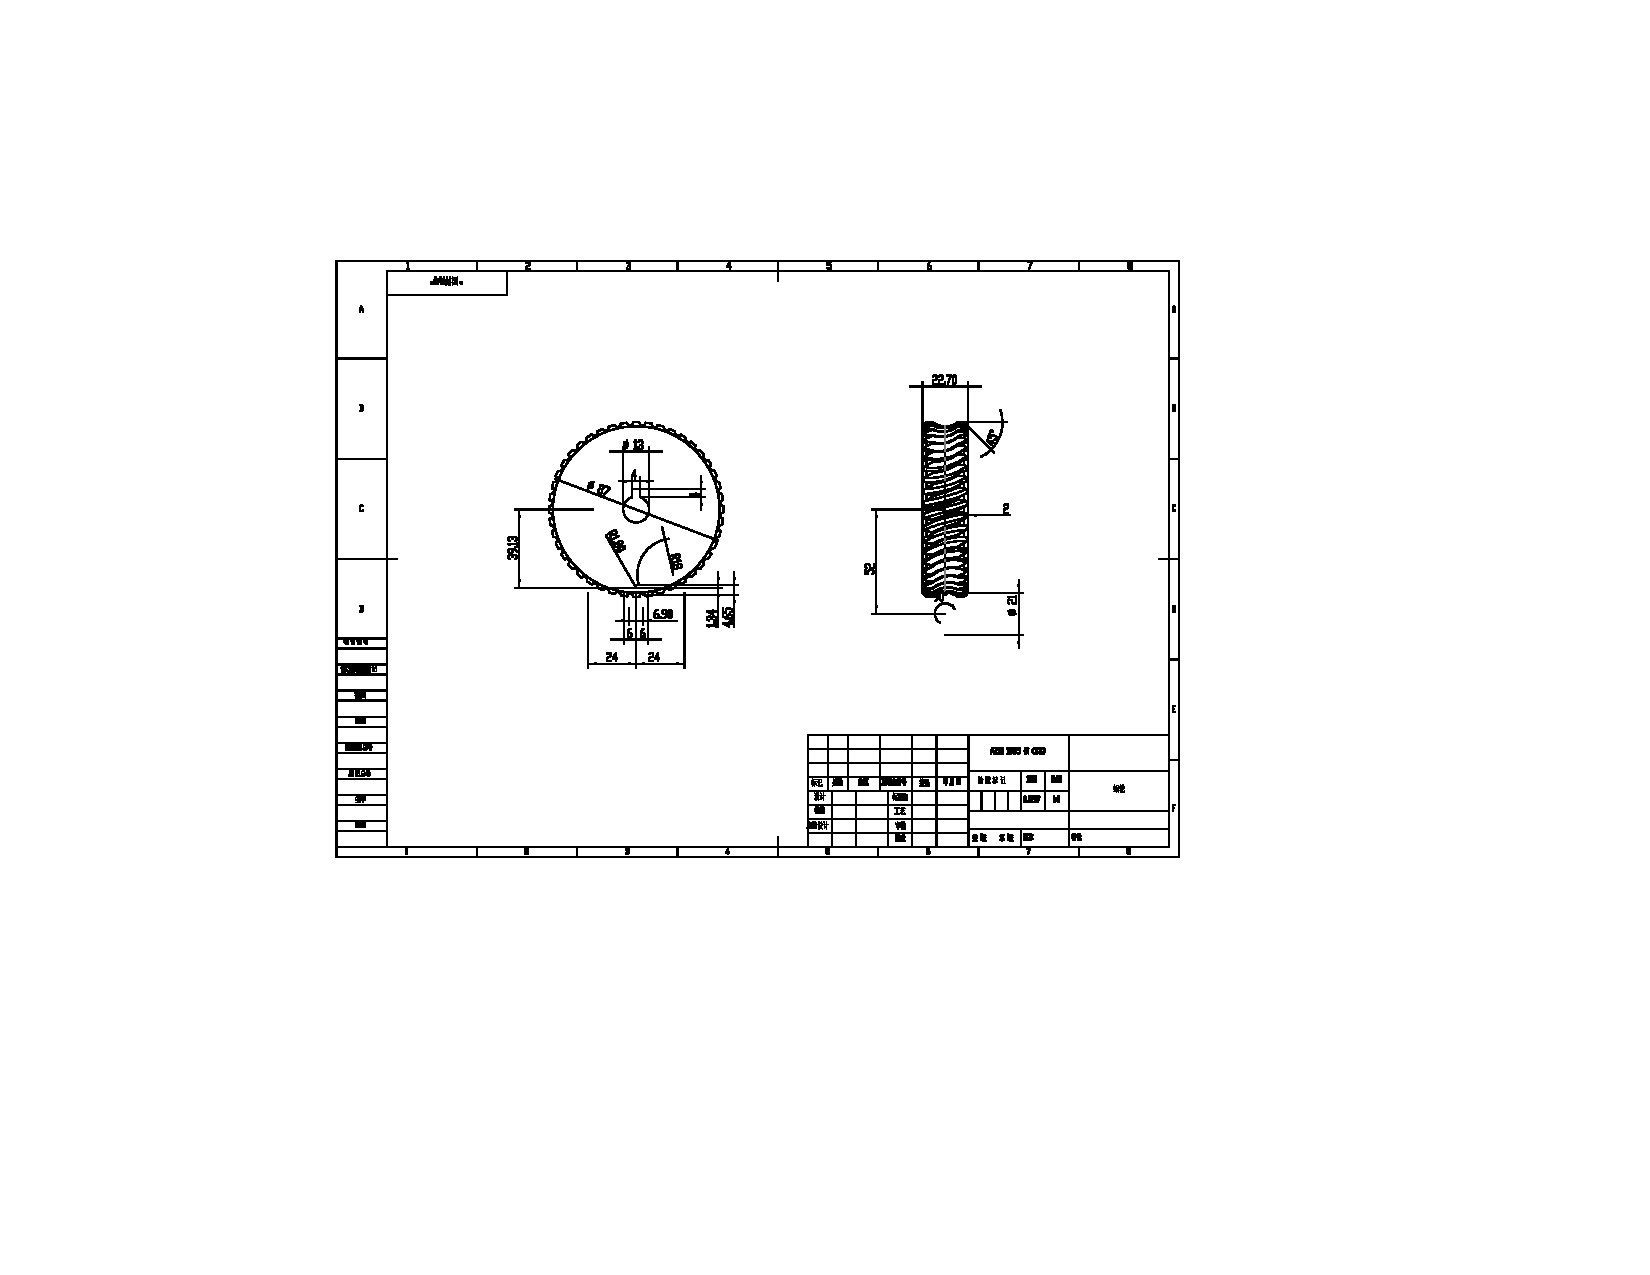
\includegraphics[height=.9\textwidth ,angle=-90]{蜗轮.pdf}
	\caption{设计图纸测试}
\end{dfigure}

\zhlipsum[1][name = aspirin]

\begin{equation}
	a^2+b^3=c^4
\end{equation}

\begin{definition}
	这是定义。\footnote{这是测试脚注。}
\end{definition}

\begin{lstlisting}[language=c++,caption=一个测试,label=mycode]
#define mian main
	\end{lstlisting}

